%!TEX root = ../../../report.tex
\section{Environment creation} % (fold)
\label{sec:environment_creation}
Besides the robot, other elements can be added to the simulated world.
From the Gazebo database, other robot models or parts (as a beer or a brick) can be inserted and used for any kind of experiments.

\begin{figure}[hb!]
  \centering
  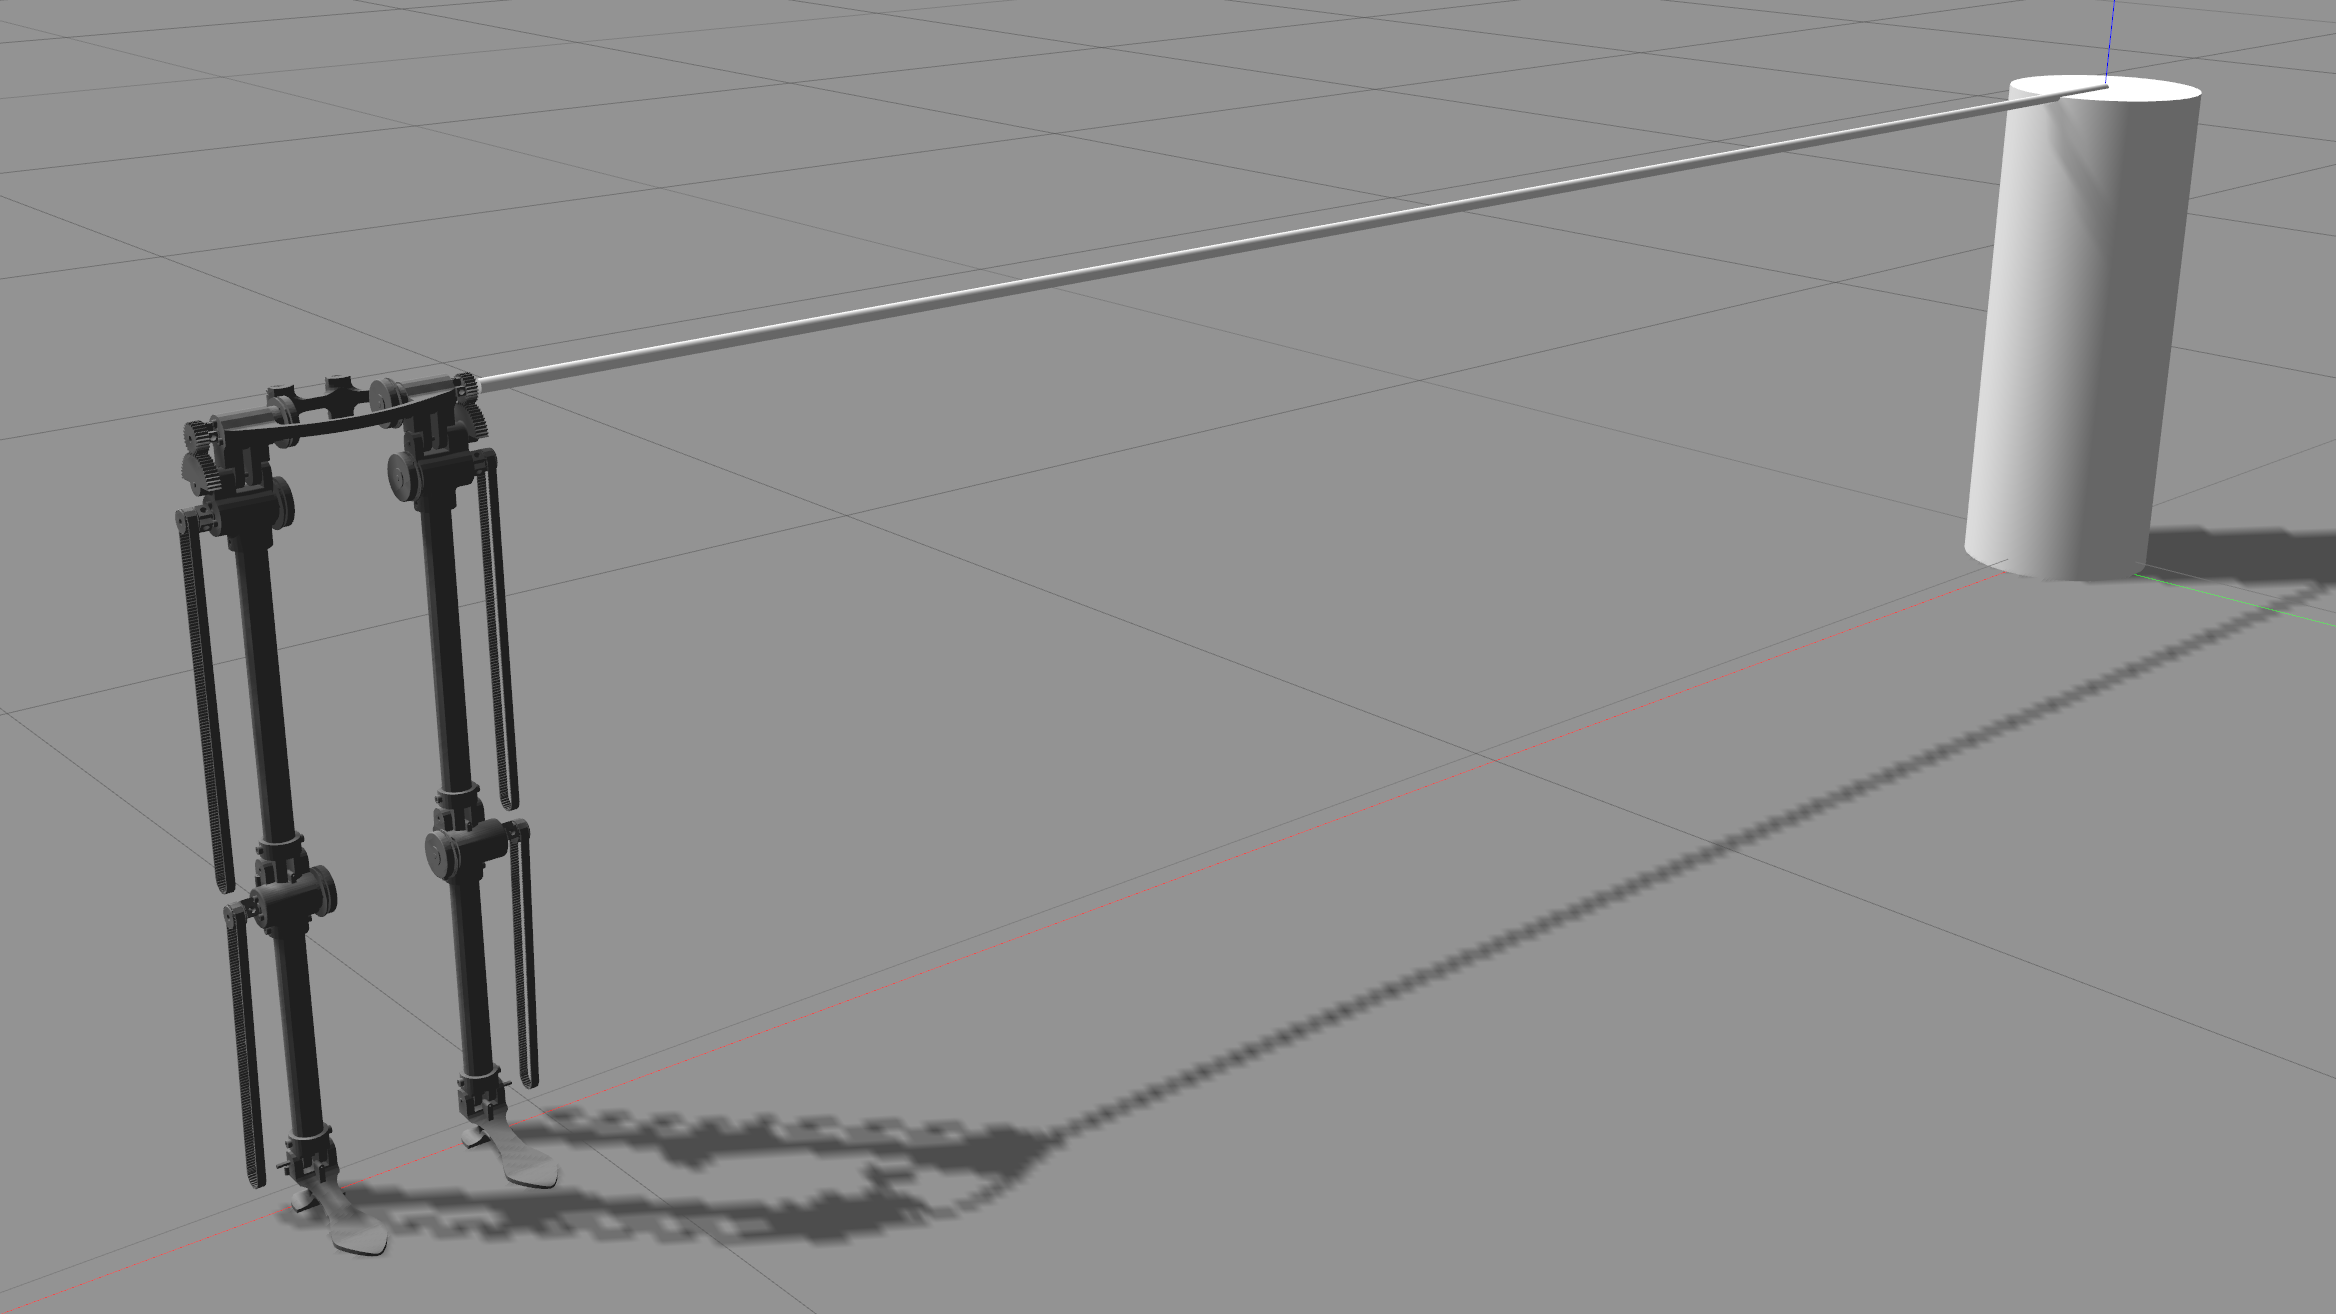
\includegraphics[width=0.75\linewidth]{figures/gazebo_rotational_holder}
  \caption{Rotational robot holder and robot}
  \label{fig:rotational_robot_holder}
\end{figure}

\hfill

In the final framework an extra tool is provided: a rotational robot holder.
It is inspired in the DACbot simulation environment in LPZ Robots, being fully parametric and reducing the degrees of freedom of the robot to constraint its motion to the scenario under study.
It can be seen in Figure \ref{fig:rotational_robot_holder}.

% section environment_creation (end)